\section{Lecture 1: Introduction}

\subsection{Some Common Operations on Signals}
%
For the sake of introducing some basic definitions with which we can gain some
physical intuition, we'll define a \textbf{signal} as a stream of information
which originates from a sensor (and isn't necessarily indexed by time), and a
\textbf{system} as an entity which processes signals and produces other signals.
%
Several types of transformation can be applied to a signal. Those that we'll find
useful in the future are given in Figure \ref{fig::lecture_1_signal_operations}.
%
\begin{figure}[!htb]
  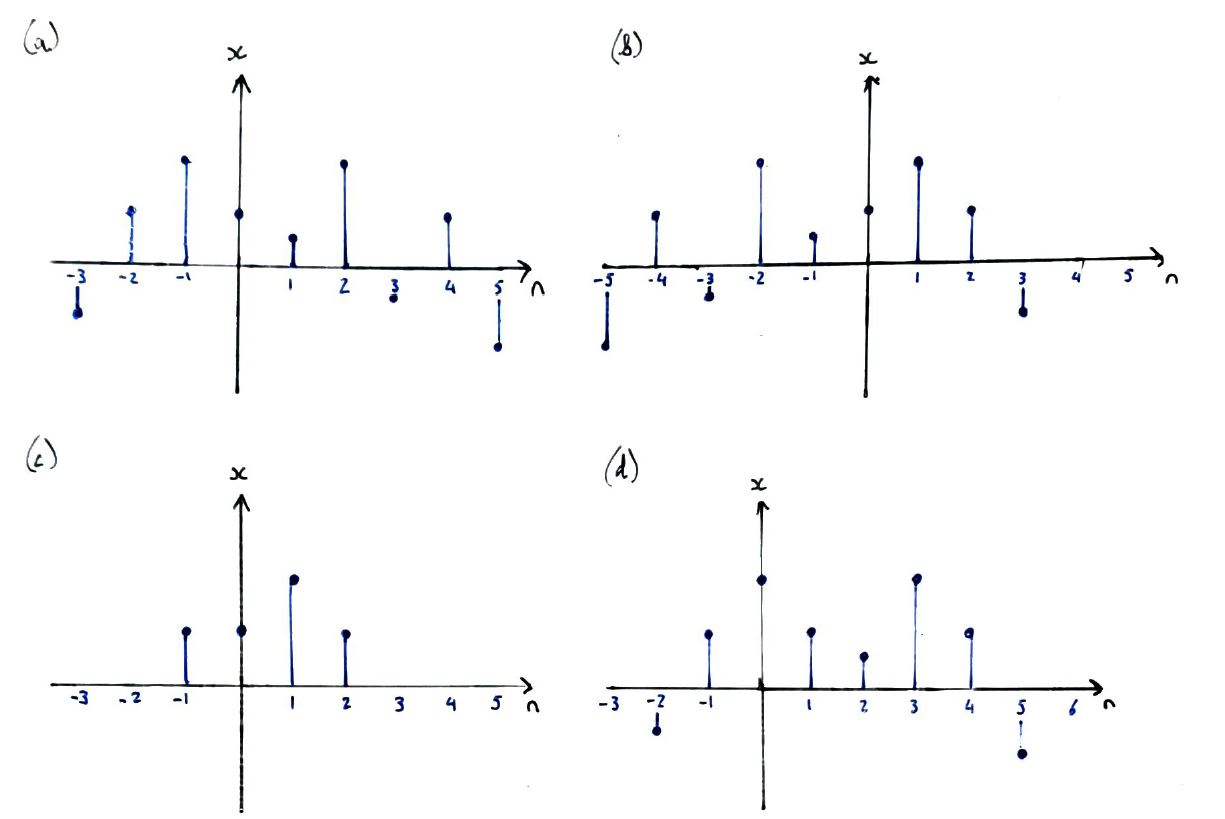
\includegraphics[width=\textwidth]{images/lecture_1_signal_operations.JPG}
  \caption{
    An example of some signals and common manipulations. (a) shows a
    signal, $x_a[n]$. (b) shows the signal from (a) having been ``reflected''
    (about the vertical axis), $x_b[n] = x_a[-n]$. (c) shows the signal from (a)
    having been ``scaled'' (in the horizontal axis), $x_c[n] = x_a[2n]$. (d) shows
    the signal from (a) having been ``shifted'' (along the horizontal axis),
    $x_d[n] = x_a[n+3]$.
  }
  \label{fig::lecture_1_signal_operations}
\end{figure}


\subsection{Compositions of Transformations}
%
The three transformations we've just discussed can be composed with general form
$n^\prime \leftarrow an + b$, where $a$ arises from the reflection and scaling (reflection
can be thought of as scaling by negative one) and $b$ arises from the shifting.
The order in which one applies these transformations is important since nonlinear algebra
is non-commutative, and can be deduced through the use of regular function composition.
Denote the reflection and scaling by $A: n\rightarrow an$ and shifting by
$B: n\rightarrow n+b$. Then,
%
\begin{displaymath}
  (B\circ A)(n) = B(an) = an + ab \,,
\end{displaymath}
%
which is clearly wrong. Exchanging the order of operations,
%
\begin{displaymath}
  (A\circ B)(n) = A(n + b) = an + b \,,
\end{displaymath}
%
as required. Consequently, transformations should be applied in the order
\textbf{shift, flip, scale}. This ordering is summarised in Figure
\ref{fig::lecture_1_transformation_order}.
%
\begin{figure}[!htb]
  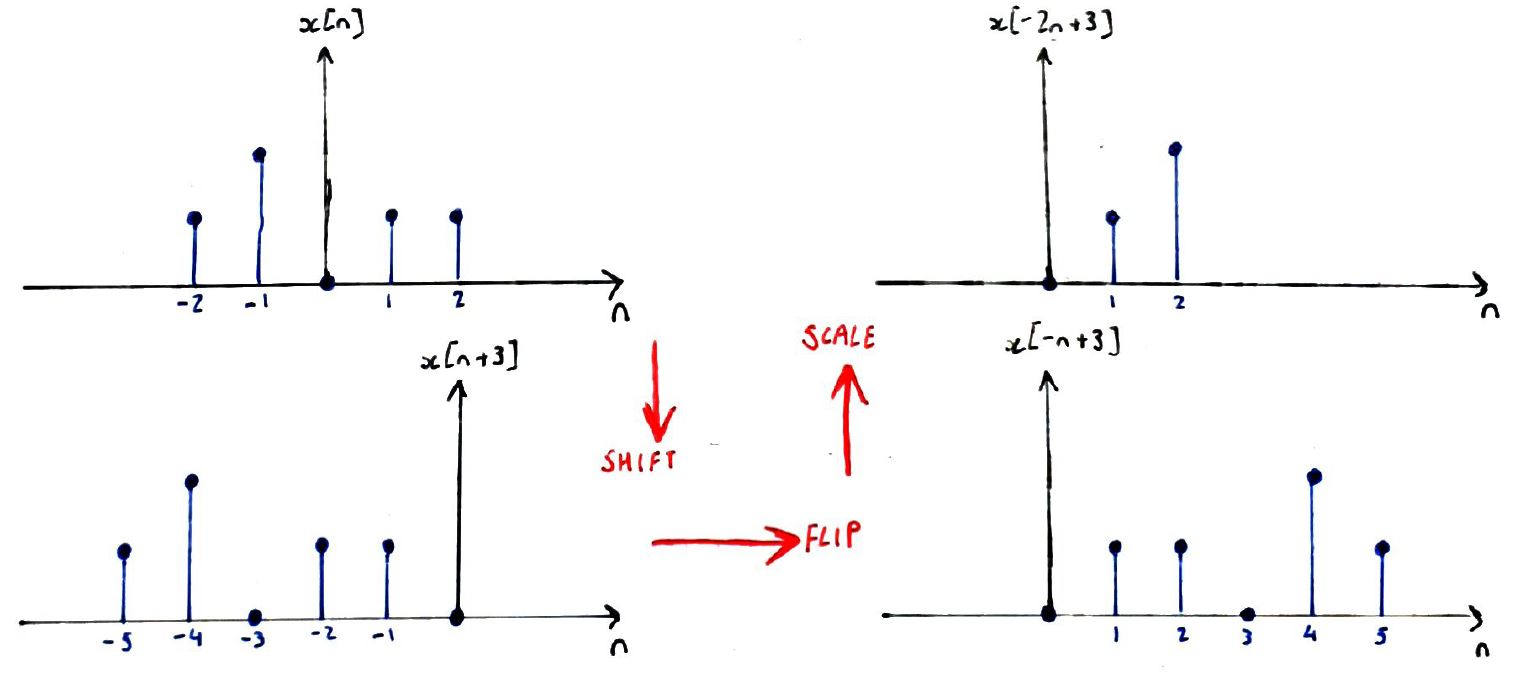
\includegraphics[width=\textwidth]{images/lecture_1_transformation_order.JPG}
  \caption{
    Ordering of transformations when dealing with a composite transformation, in
    this example $x[-2n+3]$.
    The original signal (top left) is first shifted (bottom left), reflected
    about the vertical axis (bottom right) and finally scaled (top right).
  }
  \label{fig::lecture_1_transformation_order}
\end{figure}


\subsection{Even and Odd Functions}
%
A signal is \textbf{even} if $x[n] = x[-n]$, i.e. it is symmetric about the vertical axis.
A signal is \textbf{odd} if $x[n] = -x[-n]$, i.e. it is symmetric about the function $y = -x$.
Every signal has even and odd parts, as given by the formulae:
%
\begin{align}
  \mathrm{Even}(x[n]) &= \frac{1}{2}(x[n] + x[-n]) \,, \\
  \mathrm{Odd}(x[n]) &= \frac{1}{2}(x[n] - x[-n])  \,.
\end{align}
%
The original signal can then be recovered by adding odd and even parts. Through use of the
definitions of even and odd functions, we can verify the above representations are indeed
even and odd,
%
\begin{align*}
  \mathrm{Even}(x[n]) &= \frac{1}{2}(x[n] + x[-n]) \Longrightarrow \frac{1}{2}(x[n] + x[-n]) \qquad (x[n] = x[-n])\,, \\
  \mathrm{Odd}(x[n]) &= \frac{1}{2}(x[n] - x[-n]) \Longrightarrow \frac{1}{2}(x[n] - x[-n]) \qquad (x[n] = -x[-n])\,.
\end{align*}


\subsection{Special Signals}
%
The \textbf{delta function}, $\delta[n]$, is defined as being zero at all places where its argument
is non-zero, and one where its argument is zero (see part (a) of Figure \ref{fig::lecture_1_delta_and_step}),
%
\begin{equation}
  \delta[n] = \left\{\begin{array}{ccl}
    1 & & n = 0 \\
    0 & & n \neq 0
  \end{array}\right. \,.
\end{equation}
%
Note that this is simply the Kronecker delta function, where the second argument is zero, i.e. $\delta_{n0}$.
The \textbf{step function}, $u[n]$, is defined as being zero for all negative arguments and one for
all arguments that are greater than or equal to zero (see part (b) of Figure
\ref{fig::lecture_1_delta_and_step}),
%
\begin{equation}
  u[n] = \left\{\begin{array}{ccl}
    1 & & n \geq 0 \\
    0 & & n < 0
  \end{array}\right. \,.
\end{equation}
%
\begin{figure}[!htb]
  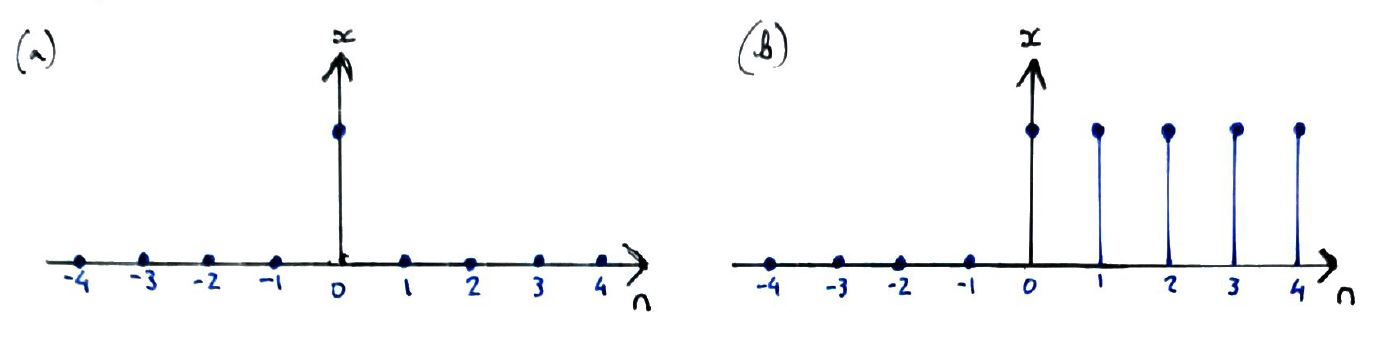
\includegraphics[width=\textwidth]{images/lecture_1_delta_and_step.JPG}
  \caption{
    The delta function (left) and step function (right).
  }
  \label{fig::lecture_1_delta_and_step}
\end{figure}
%
The step function can be written in terms of an infinite sum over shifted delta functions,
%
\begin{equation}
  u[n] = \delta[n] + \delta[n-1] + \delta[n-2] + \hdots = \sum_{k=0}^\infty \delta[n-k]
\end{equation}
%
In continuous-variable calculus, it can be shown that the Heaviside function, $H(t)$, (the continuous
analogue of the step function) can be written as an integral over the impulse response,
%
\begin{displaymath}
  H(t) = \int^t_{-\infty} \dx{\tau}\delta(t) \,.
\end{displaymath}
%
This integral is zero until $\tau = t$, at which point it becomes, and remains, one. In a similar
fashion, we can write the step function as a ``discrete integral'', i.e. a summation,
%
\begin{equation}
  u[n] = \sum_{k=-\infty}^n \delta[k] \,.
\end{equation}
%
One can conversely think of the delta function as the discrete derivative of the step function,
%
\begin{equation}
  \delta[n] = u[n] - u[n-1] \,,
\end{equation}
%
although note that in the discrete case, the derivative is well-defined, in contrast to the continuous
case where the derivative at the transition is undefined.\\
%
In the same way as we have created the step function from an infinite sum of shifted delta functions,
we can write any signal as an infinite sum of shifted and scaled delta functions (see Figure
\ref{fig::lecture_1_sum_of_deltas}),
%
\begin{equation}
  x[n] = \sum_{k=-\infty}^\infty \delta[n-k] x[k]
\end{equation}
%
This seems like something of a convoluted way to write out a function, but it simply allows us to
break a signal down into a sum of its component pieces using the ``sifting'' or ``sampling'' property
of the delta function, which allows us to parse out a part of a signal that we want.
%
\begin{figure}[!htb]
  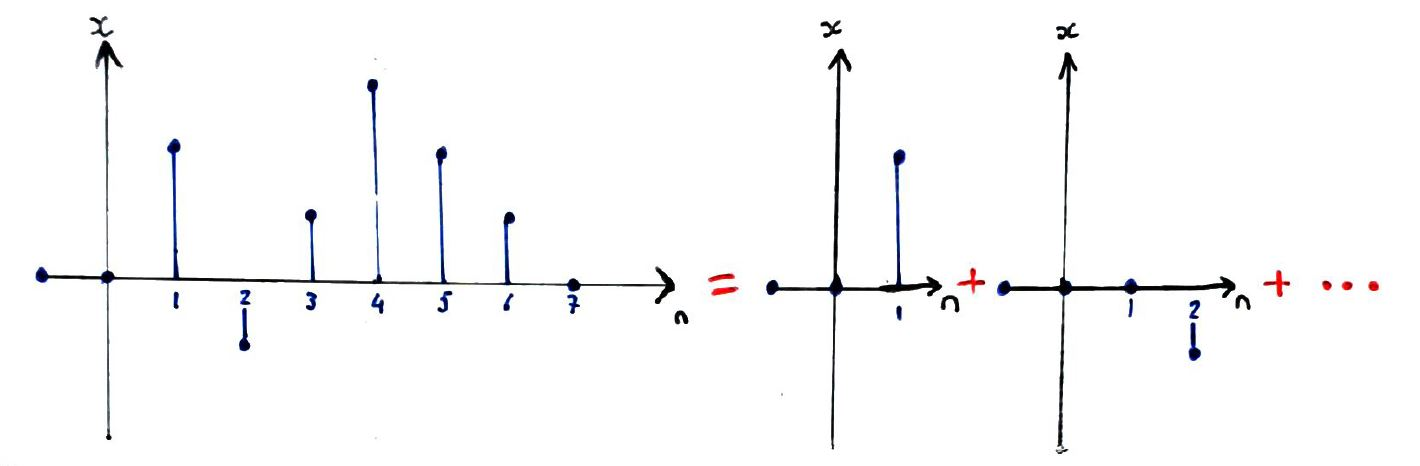
\includegraphics[width=\textwidth]{images/lecture_1_sum_of_deltas.JPG}
  \caption{
    A signal can be written as a sum of shifted and scaled delta functions.
  }
  \label{fig::lecture_1_sum_of_deltas}
\end{figure}

\subsection{Complex Number Review}
%
Foregoing the basic introduction to complex numbers, we'll just recap by taking a specific
example whose form it will prove useful to know about in the future. Consider $x[t] = C\ex{at}$,
where $C,a\in \mathbb{C}^2$. Writing $C = |C|\ex{\im\theta}$ in
polar form and $a = r + \im\omega_0$ in rectilinear form, we can form the expression
%
\begin{align*}
  x[t] &= C\ex{at} = |C|\ex{\im\theta}\ex{rt}\ex{\im\omega_0 t} = |C|\ex{rt}\ex{\im(\theta + \omega_0 t)} \\
  &= |C|\ex{rt}\left[ \cos(\omega_0 t + \theta) + \im\sin(\omega_0 t + \theta) \right]
\end{align*}
%
Taking the real part of $x[t]$, we see that the function is the cosine whose amplitude is bounded by the
exponential $|C|\ex{rt}$, which is either increasing or decreasing depending on whether $r$ is positive
or negative, respectively. The imaginary part simply exchanges the cosine for a sine.
We'll encounter many signals of this form, and referring back to its behaviour
will prove useful. It is graphed in Figure \ref{fig::lecture_1_complex_numbers}.
%
\begin{figure}[!htb]
  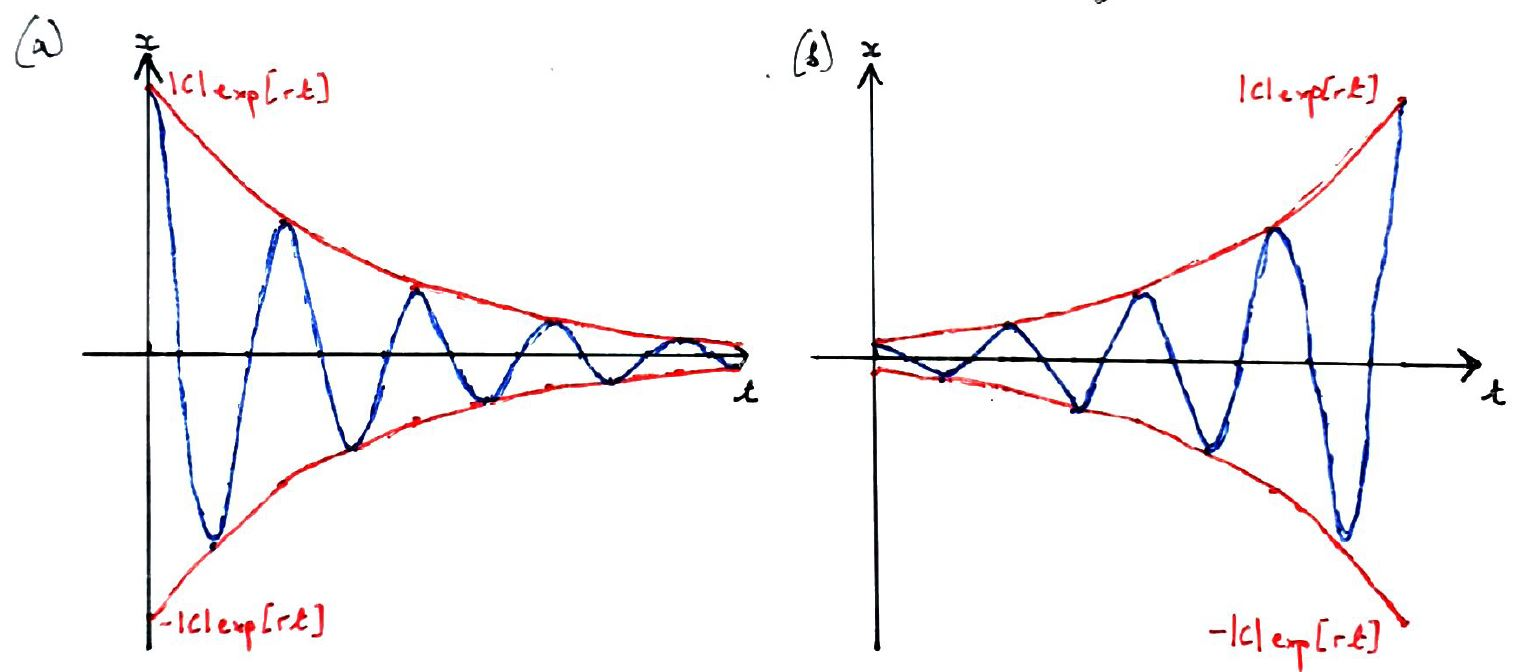
\includegraphics[width=\textwidth]{images/lecture_1_complex_numbers.JPG}
  \caption{
    The real part of
    $|C|\ex{rt}\left[ \cos(\omega_0 t + \theta) + \im\sin(\omega_0 t + \theta) \right]$
    when $r < 0$ (left) and $r > 0$ (right). The red lines define the bounding exponentials.
  }
  \label{fig::lecture_1_complex_numbers}
\end{figure}

\subsection{Periodicity in Discrete Time}
%
Consider the function $\ex{\im\omega_0 n}$, a phasor rotating around the complex plane with frequency
$\omega_0$. Adding a term to $\omega_0$ results in a phasor of higher frequency. For the continuous
time case, the function $\ex{\im(\omega_0 + 2\pi)n}$ is a phasor whose frequency is $2\pi$ higher
than $\ex{\im\omega_0 n}$. However, for the discrete time case, we have that $n\in\mathbb{N}$.
Factoring our phasor,
%
\begin{displaymath}
  \ex{\im(\omega_0 + 2\pi)n} = \ex{\im\omega_0n}\ex{\im 2\pi n} = \ex{\im\omega_0n} \,.
\end{displaymath}
%
For a discrete time system, adding $2\pi$ to any frequency returns the same frequency
\footnote{
  Note that this is different in the continuous time case where
  $\ex{\im\omega t} \neq \ex{\im(\omega + 2\pi)t}$ since $t\in\mathbb{R}$. So while equality
  holds when $t$ coincides with integer values, it must hold $\forall t$ if the function is to
  be $2\pi$-periodic. Consequently, the continuous time phasor is not $2\pi$-periodic like
  the discrete time case.
}, and consequently there's an upper bound on the frequencies we can explore in discrete
time -- that upper bound is $\pi$ (i.e. two samples per period) since this results in
%
\begin{displaymath}
  \ex{\pi n} = \left\{\begin{array}{ccl}
  1 & & n\hspace{1mm}\mathrm{even} \\
  -1 & & n\hspace{1mm}\mathrm{odd} \\
  \end{array}\right. \,,
\end{displaymath}
%
(see Figure \ref{fig::lecture_1_discrete_sampling}) the highest frequency with which we can recover
a sinusoid -- a sampling frequency higher than this will result in aliasing (to be covered in a
later lecture). 
%
\begin{figure}[!htb]
  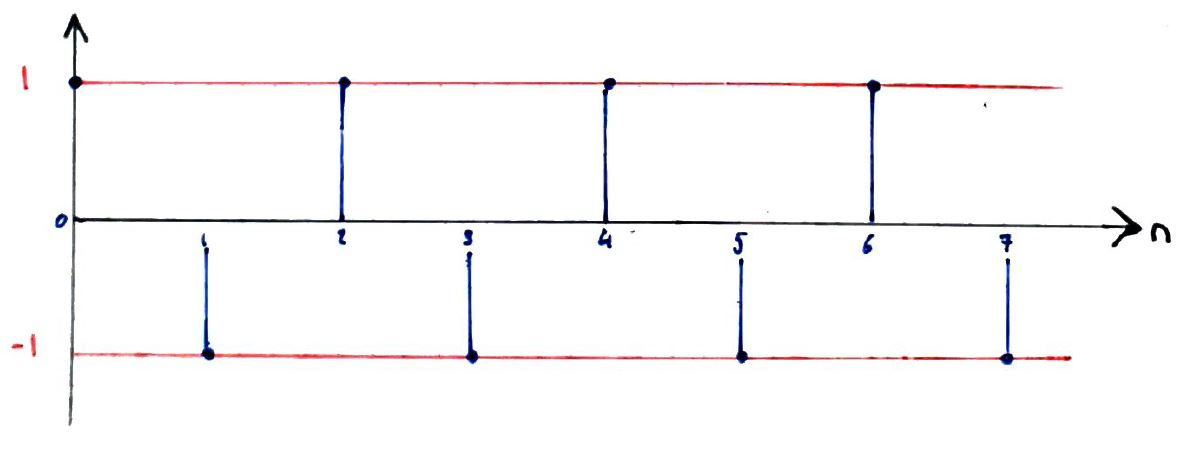
\includegraphics[width=\textwidth]{images/lecture_1_discrete_sampling.JPG}
  \caption{
    A discretely sampled sinusoid of frequency $\pi$. Sampling the upper and lower bounds of
    the sinusoid allows for its reconstruction. Were the sinusoid a higher frequency, two samples
    could not be made per cycle.
  }
  \label{fig::lecture_1_discrete_sampling}
\end{figure}
%
One needs to be careful in assessing whether a signal is periodic in discrete time.
We need to answer when is $\ex{\im\omega_0 n}$ periodic in discrete time. By
the periodicity condition, $\ex{\im\omega_0(n+N)} = \ex{\im\omega_0n}$ for the signal
to be periodic with period $N\in\mathbb{N}$. Factoring our expression,
%
\begin{displaymath}
  \ex{\im\omega_0(n+N)} = \ex{\im\omega_0n}\ex{\im\omega_0N} \,,
\end{displaymath}
%
meaning that we require this final term to equate to one, which is satisfied when $\omega_0N$
is some multiple of $2\pi$, i.e.
%
\begin{displaymath}
  \omega_0N = 2\pi k, \qquad k\in\mathbb{N} \,.
\end{displaymath}
%
This then leads us to
%
\begin{displaymath}
  \omega_0 = \frac{2\pi k}{N} \quad\rightarrow\quad N = \frac{2\pi k}{\omega_0} \,,
\end{displaymath}
%
i.e. $N$ must be some integer multiple of $\frac{2\pi}{\omega_0}$.
%
\begin{exmp}
  Consider $x[n] = \cos[\frac{4\pi}{5}n]$.
  \begin{displaymath}
    N = \frac{2\pi k}{\omega_0} = \frac{10\pi k}{4\pi} = \frac{5}{2}k \,.
  \end{displaymath}
  Since $N,k\in\mathbb{N}$, we find that $k=2, N=5$ and the signal is periodic with
  period 5.
\end{exmp}
\begin{exmp}
  Consider $x[n] = \cos[7n]$. In continous time, this function is periodic with period
  $\frac{2\pi}{7}$. However, in discrete time,
  \begin{displaymath}
    N = \frac{2\pi k}{\omega_0} = \frac{2\pi k}{7} \,.
  \end{displaymath}
  But there is no integer $k$ which yields $N\in\mathbb{N}$ ($\pi$ is irrational, and by
  definition can't be represented as a fraction of integers), and so the signal is not
  periodic in discrete time.
\end{exmp}


